\documentclass{article}
\usepackage[pdftex]{graphicx}
%\usepackage[latin1]{inputenc}
\usepackage[utf8]{inputenc}

%Bordas da página
\usepackage{setspace}
\usepackage[inner=30mm,outer=20mm,top=30mm,bottom=20mm]{geometry}

%Fonte arial
\renewcommand{\rmdefault}{phv}

%layout
\pdfpagewidth 210mm
\pdfpageheight 297mm
%\inglespacing
\onehalfspacing
%\doublespacing
%\topmargin 0in
%\headheight 0in
%\headsep 0in
%\textheight 9in
%\textwidth 6.5in
%\oddsidemargin 0in
%\evensidemargin 0in

%To use \toprule, ...
\usepackage{booktabs}

\usepackage{multirow}

\usepackage{color}

\title{Trabalho Predição\\
   Mineração de Dados}

\author{Pedro Batista - pedro@ufpa.br}

\begin{document}

\maketitle

\section{A base de dados}
Inicialmente testes realizados na base de dados mostraram resultados muito ruins.
Para tentar melhorar o resultado, analisamos o fluxo plotado em função da data,
mostrado na Figura~\ref{fig:data}. Esse gráfico nos mostrou um padrão anual, e
que varia de acordo com os meses. Desta forma, plotamos na Figura~\ref{fig:fluxo_mes},
os dados de forma que o fluxo está somado em cada mês. Onde podemos notar, que o fluxo
se repete.

\begin{figure}[h]
   \centering
   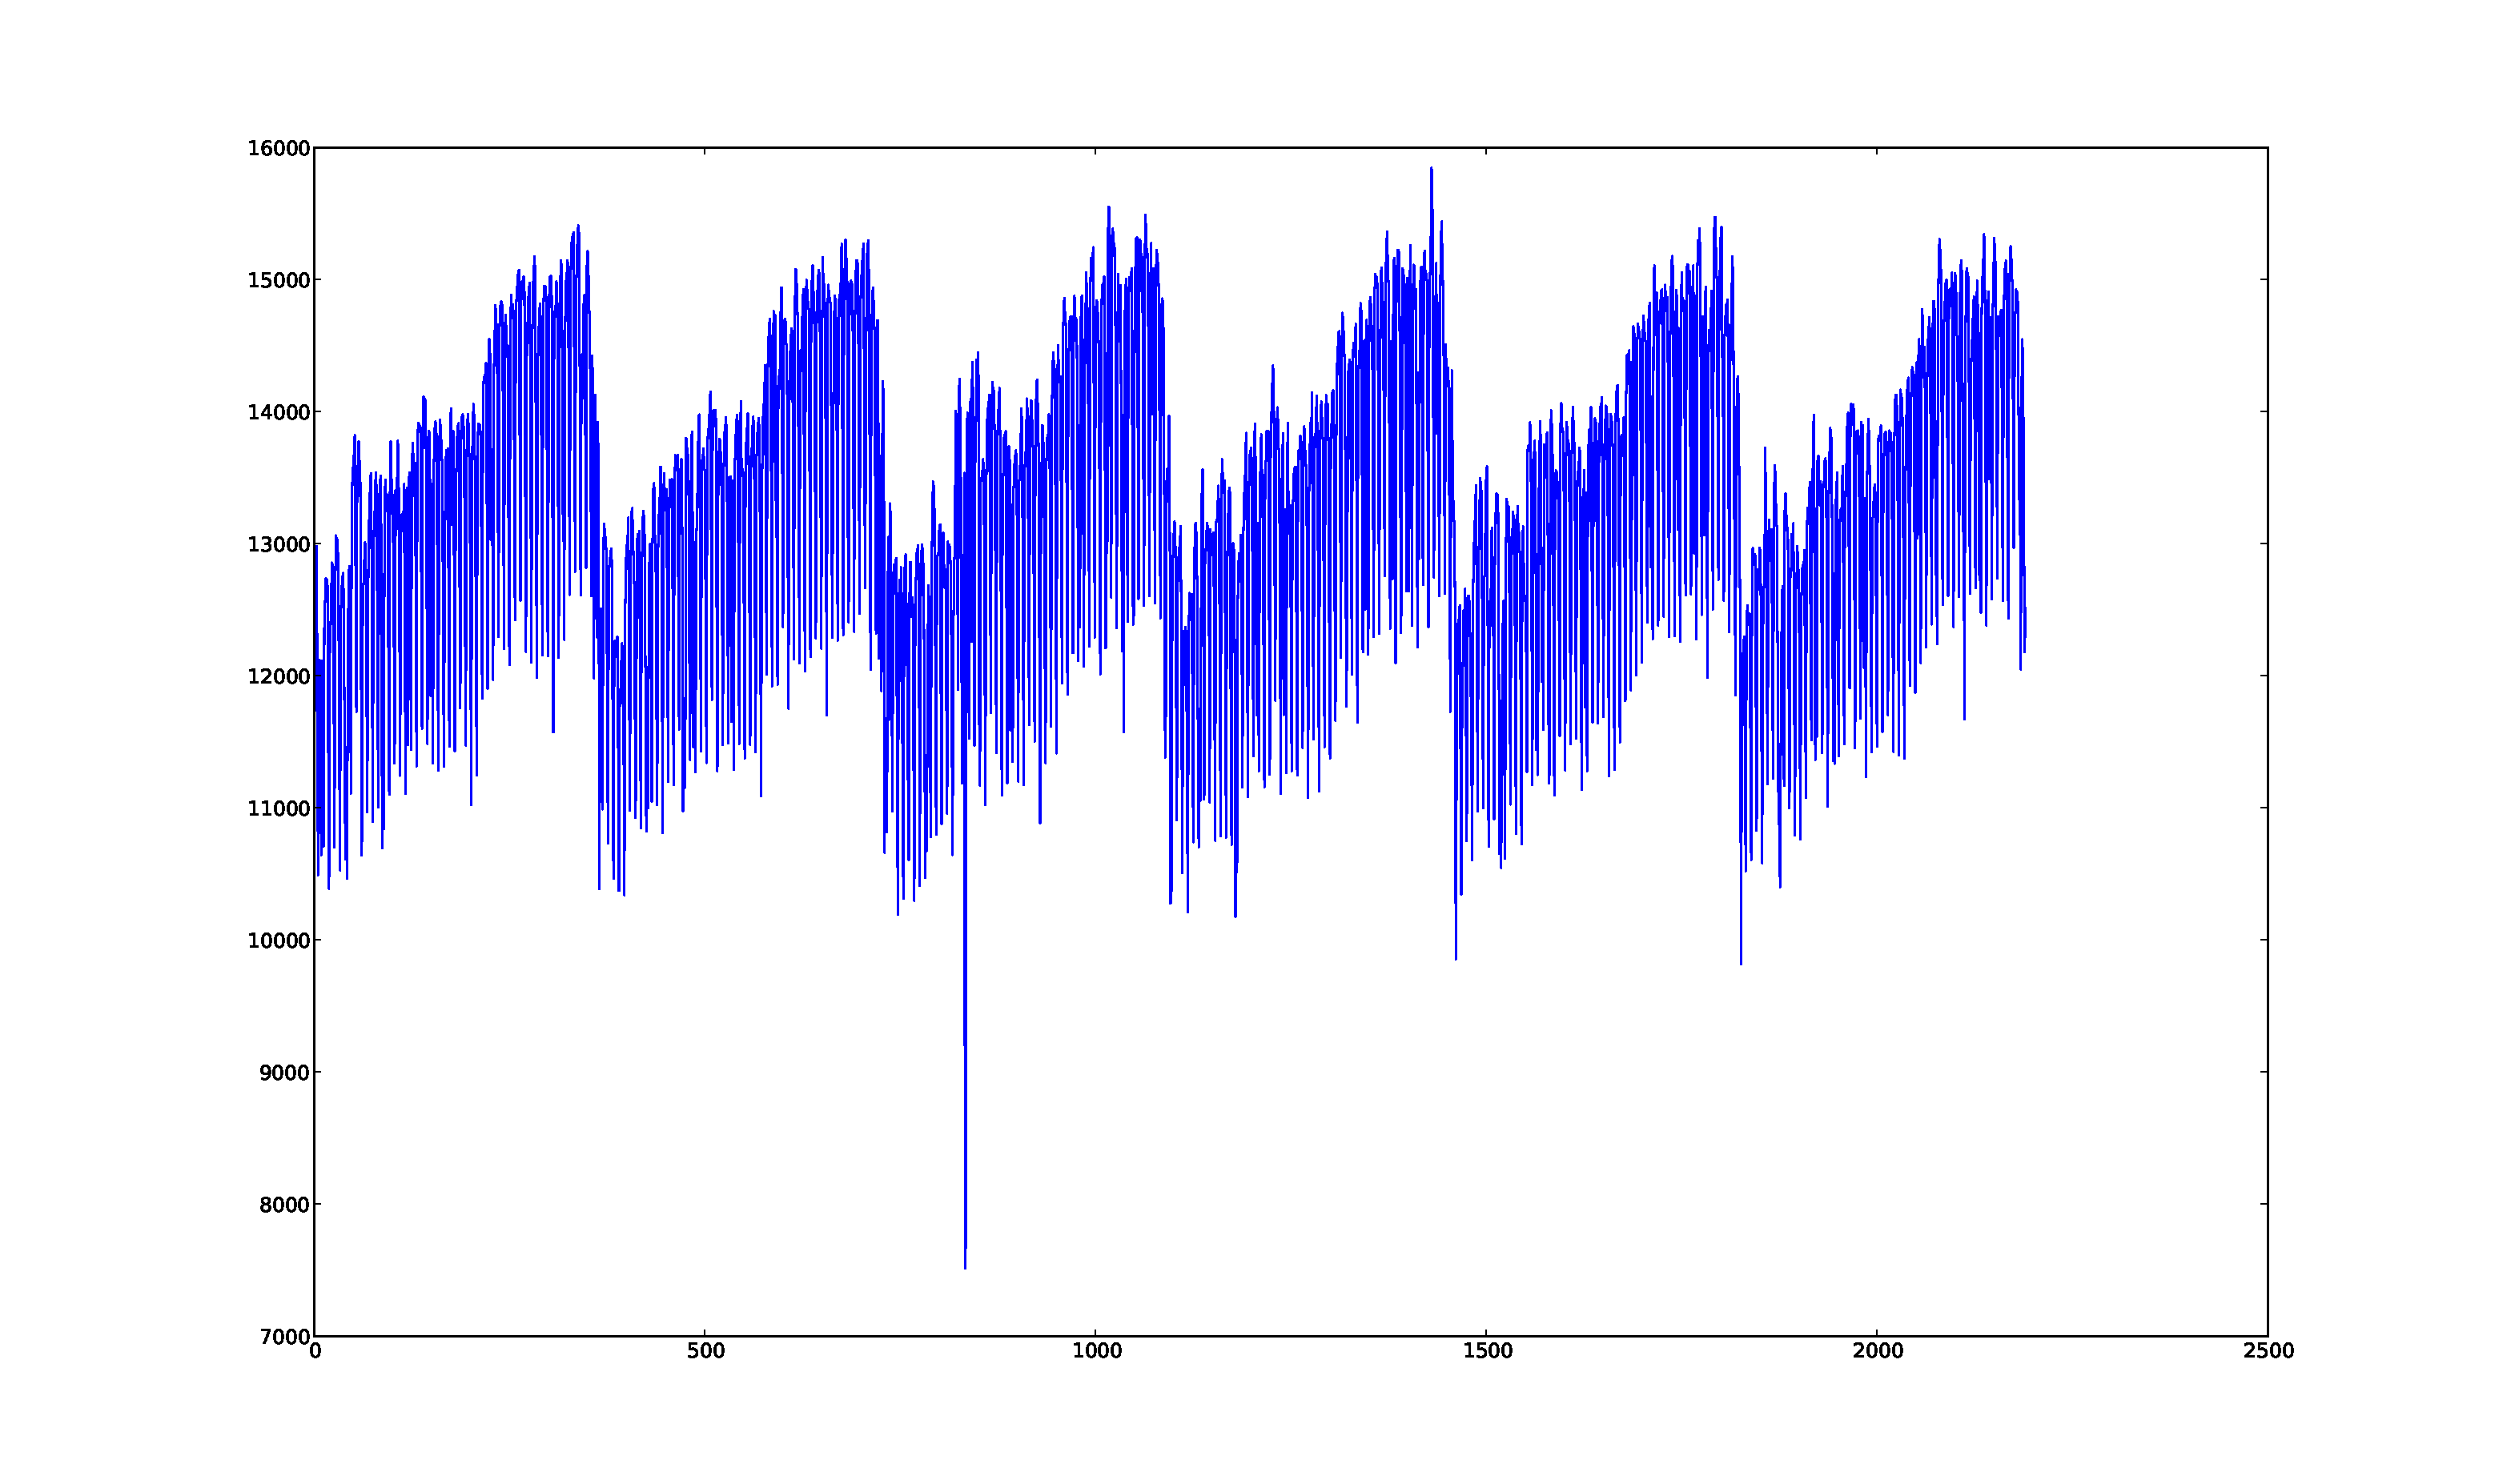
\includegraphics[height=9cm]{fluxo_data}
   \caption{Fluxo plotado em função da data.}
   \label{fig:data}
\end{figure}

\begin{figure}[h]
   \centering
   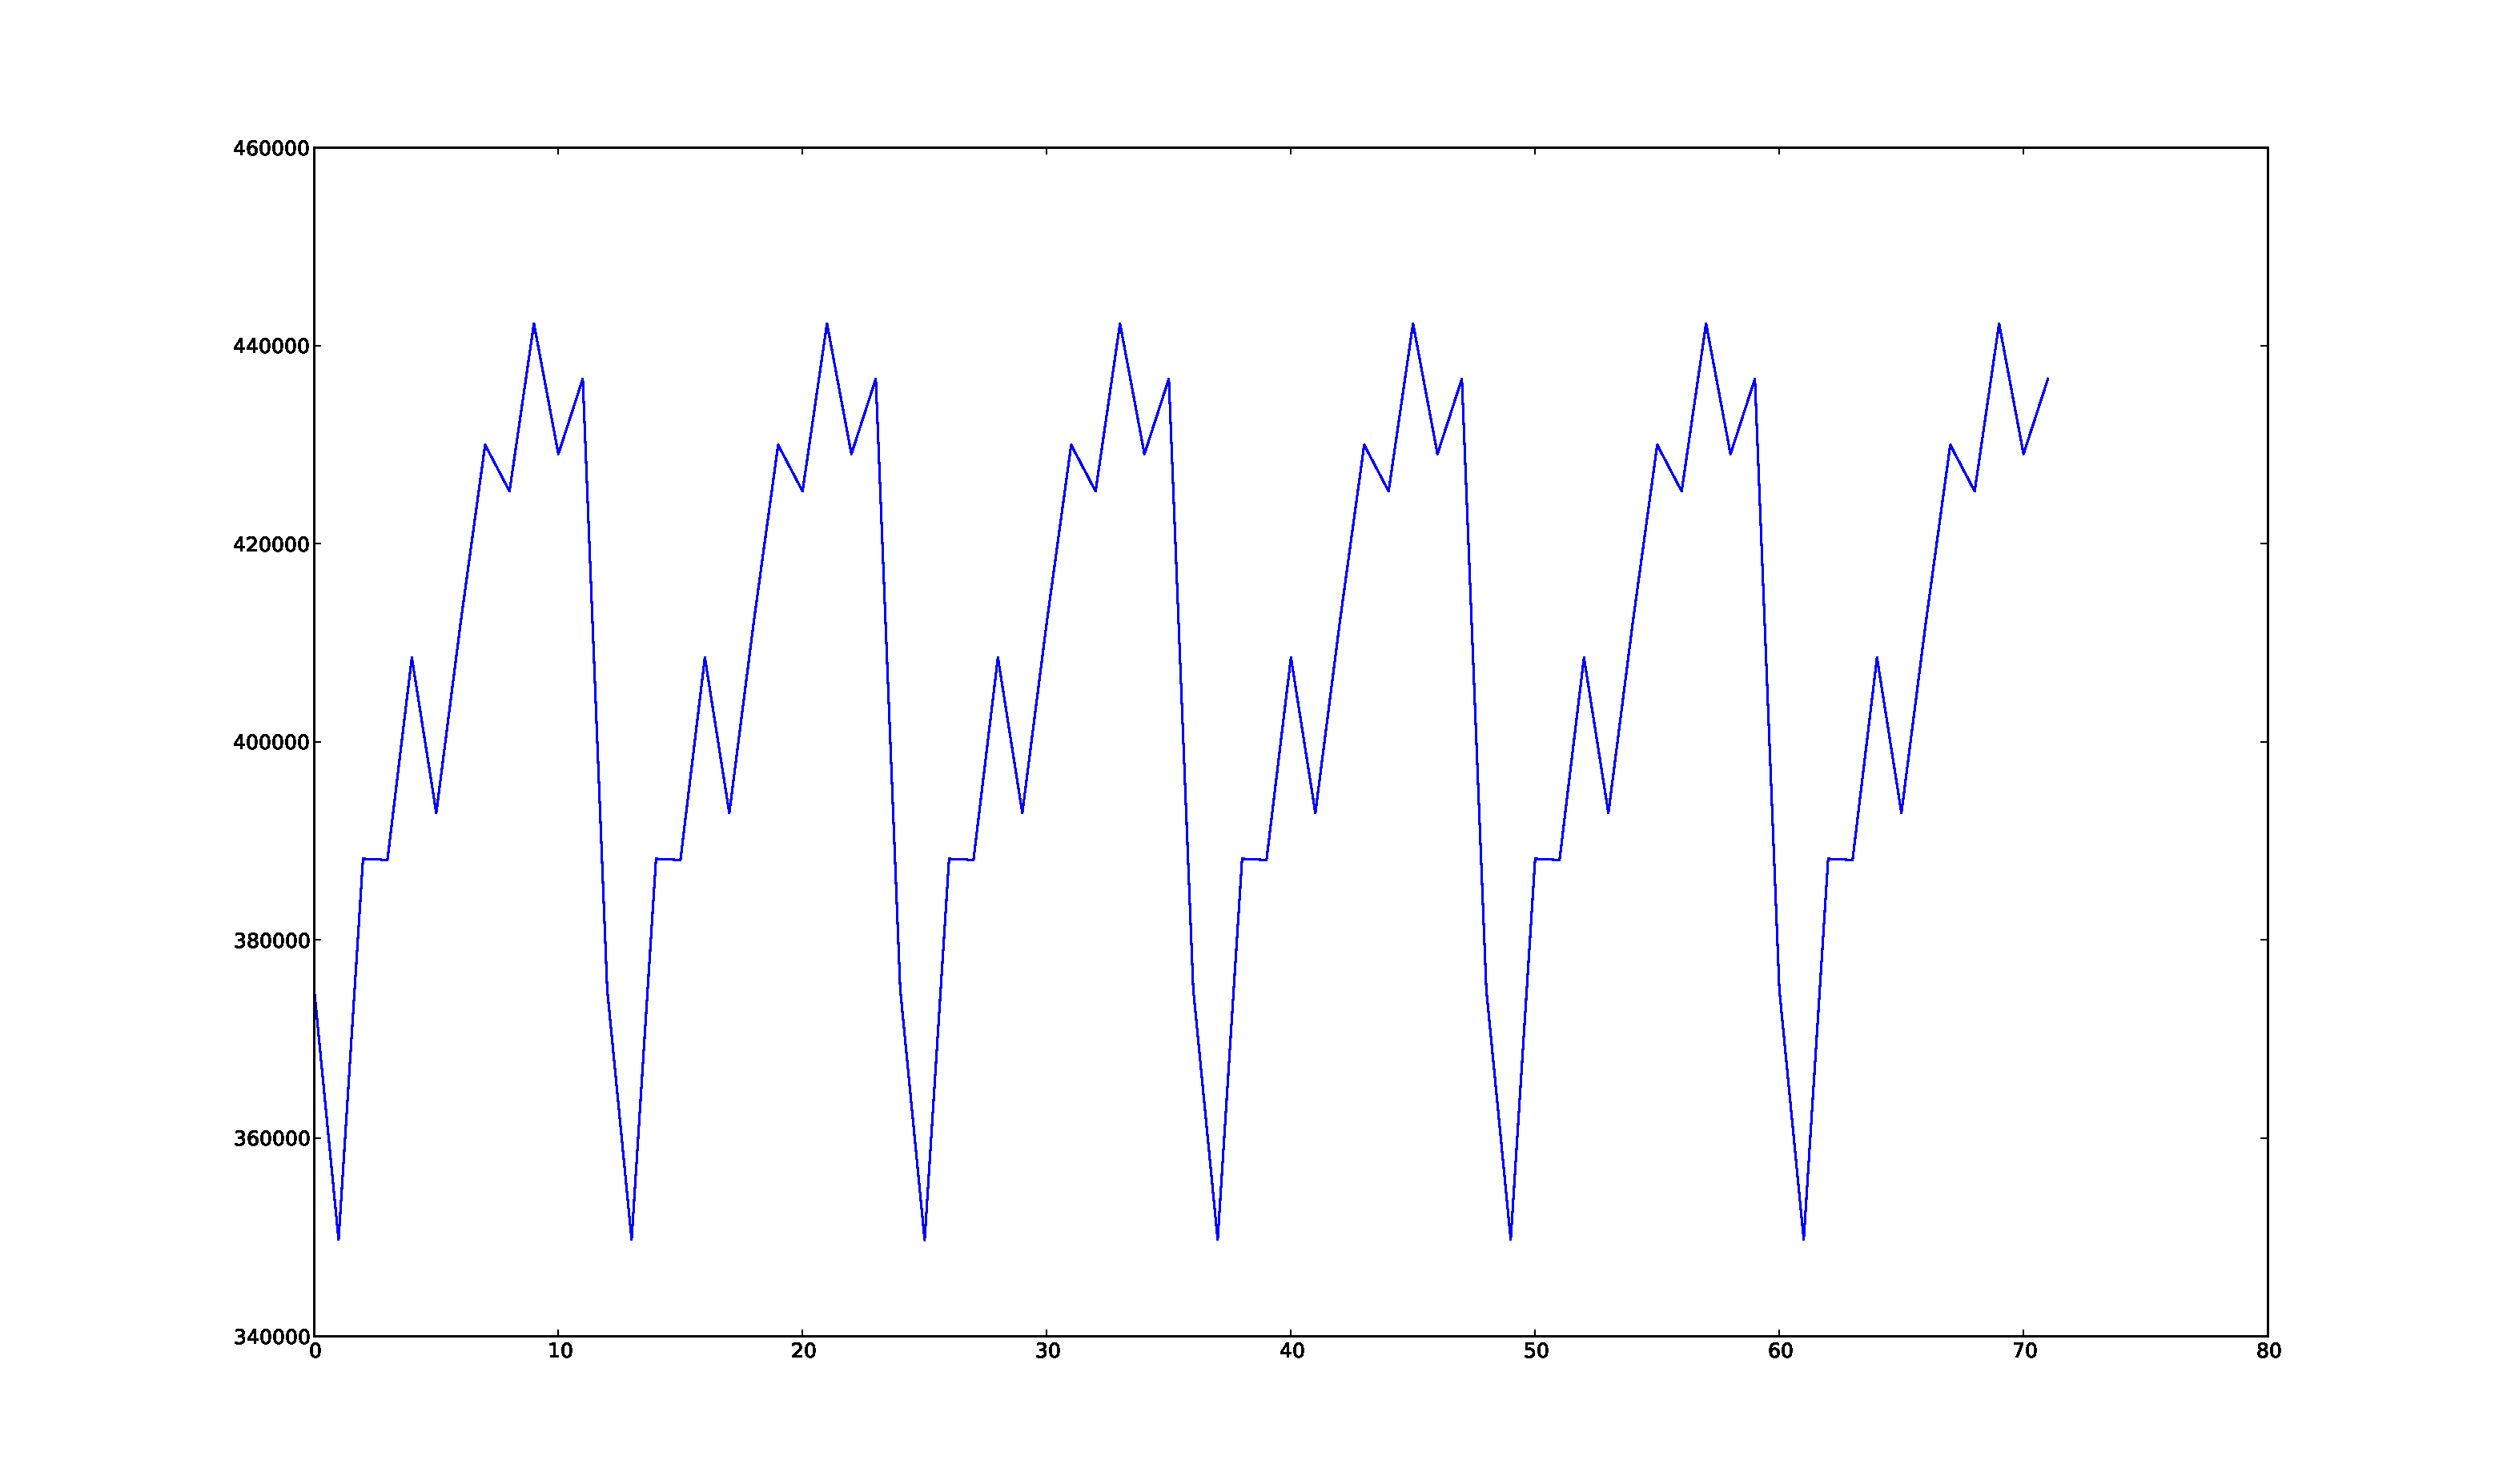
\includegraphics[height=9cm]{fluxo_mes}
   \caption{Fluxo somado por mês.}
   \label{fig:fluxo_mes}
\end{figure}

\section{Resultados}

O algoritmo de Rede Neural Multi-camada, foi então aplicado a base de dados de modo que,
a informação do dia da semana foi ignorada, assim como a informação do ano. O fluxo
original foi somando em cada mês, desta forma, a base conhecida pelo algoritmo continha,
apenas a informação número do mês e fluxo correspondente.

Para o teste com 30 dias (testado com 31 dias, mês de dezembro), foi utilizada para teste,
os dados de dezembro de 2007 e todo o resto para treino. Para o teste com 6 meses, os últimos
seis meses de 2007 foram utilizados para teste e o resto para treino. O teste anual foi realizado
com os dados do ano de 2007 e o outros para treino.

Para a RN Multi-camada, foram utilizadas, 20 camadas, taxa de aprendizagem de 0.1 e no máximo
500000 épocas para o treino. Os resultados são mostrados na Tabela~\ref{tab:results}.

\begin{table}
   \begin{tabular}{c | p{2.5cm} p{2.5cm} p{3cm} p{2.5cm}}
   \toprule
   &Mean absolute error & Root mean squared error & Relative absolute error & Root relative squared error \\\midrule
   1 mês & 4.6171 & 4.6171 & 0.0151\% & 0.0151\% \\\midrule
   6 meses & 0.9032 & 1.1745 & 0.0036\% & 0.0044\% \\\midrule
   1 ano & 2.6945 & 3.0271 & 0.0117\% & 0.0112\% \\\midrule
   \end{tabular}
   \caption{Resultados}
   \label{tab:results}
\end{table}

\end{document}
